%-------------------------------------------------------
\begin{frame}{Introduction}{A general view about the Data Mining process}
%-------------------------------------------------------
	\begin{centering}
		\vspace{0.2cm}
		\hspace{-0.2cm}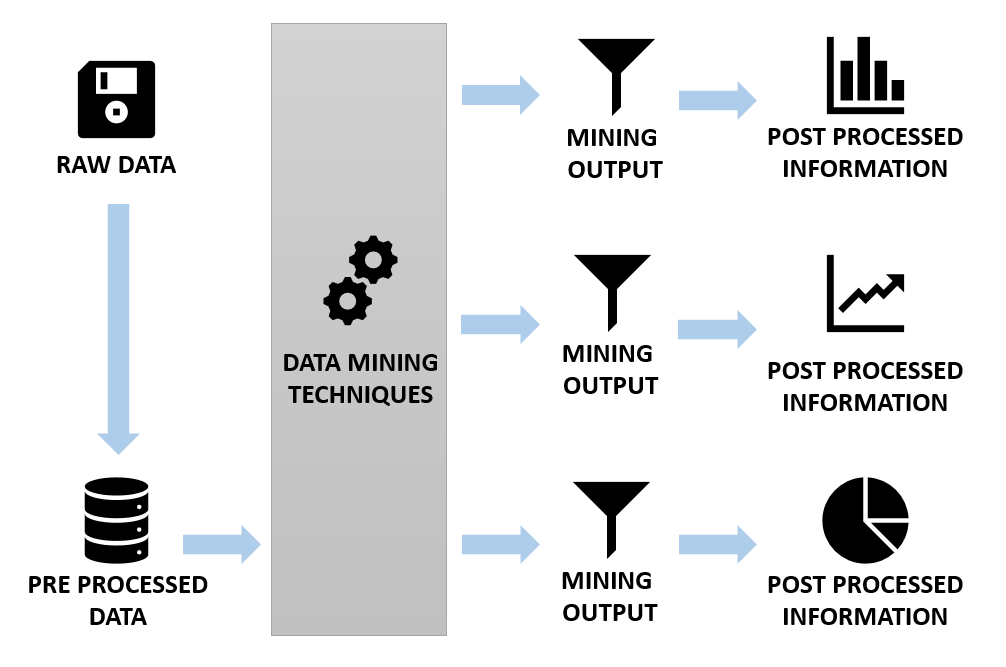
\includegraphics[scale=0.25]{img1_noback.png}
	\end{centering}
\end{frame}

%-------------------------------------------------------
\begin{frame}{Introduction}{The choice of appropriate technologies: picking the right tools}
%-------------------------------------------------------

	\begin{block}{}
	    \begin{itemize}
		    \item<1-> \alert{Data Processing}: \hspace{0.2cm} 
\includegraphics[scale=0.18, trim=0 0.8cm 0 0]{../thesis/img/mongodb.png} \\\vspace{0.2cm} \emph{New tech, noSQL paradigm, \textcolor{cyan}{good skill to learn!}}
		    \item<2-> \alert{Data Mining Algorithms}: \hspace{0.2cm} 
\includegraphics[scale=0.16, trim=0 3.2cm 0 0]{../thesis/img/weka_noback.png}  \\\vspace{0.35cm} \emph{Open source data mining software/framework;} \\\vspace{0.2cm}
			\item<3-> \alert{Visualization Techniques}: \hspace{0.2cm} 
\includegraphics[scale=0.18, trim=0 2cm 0 0]{../thesis/img/R.png} \hspace{0.4cm} 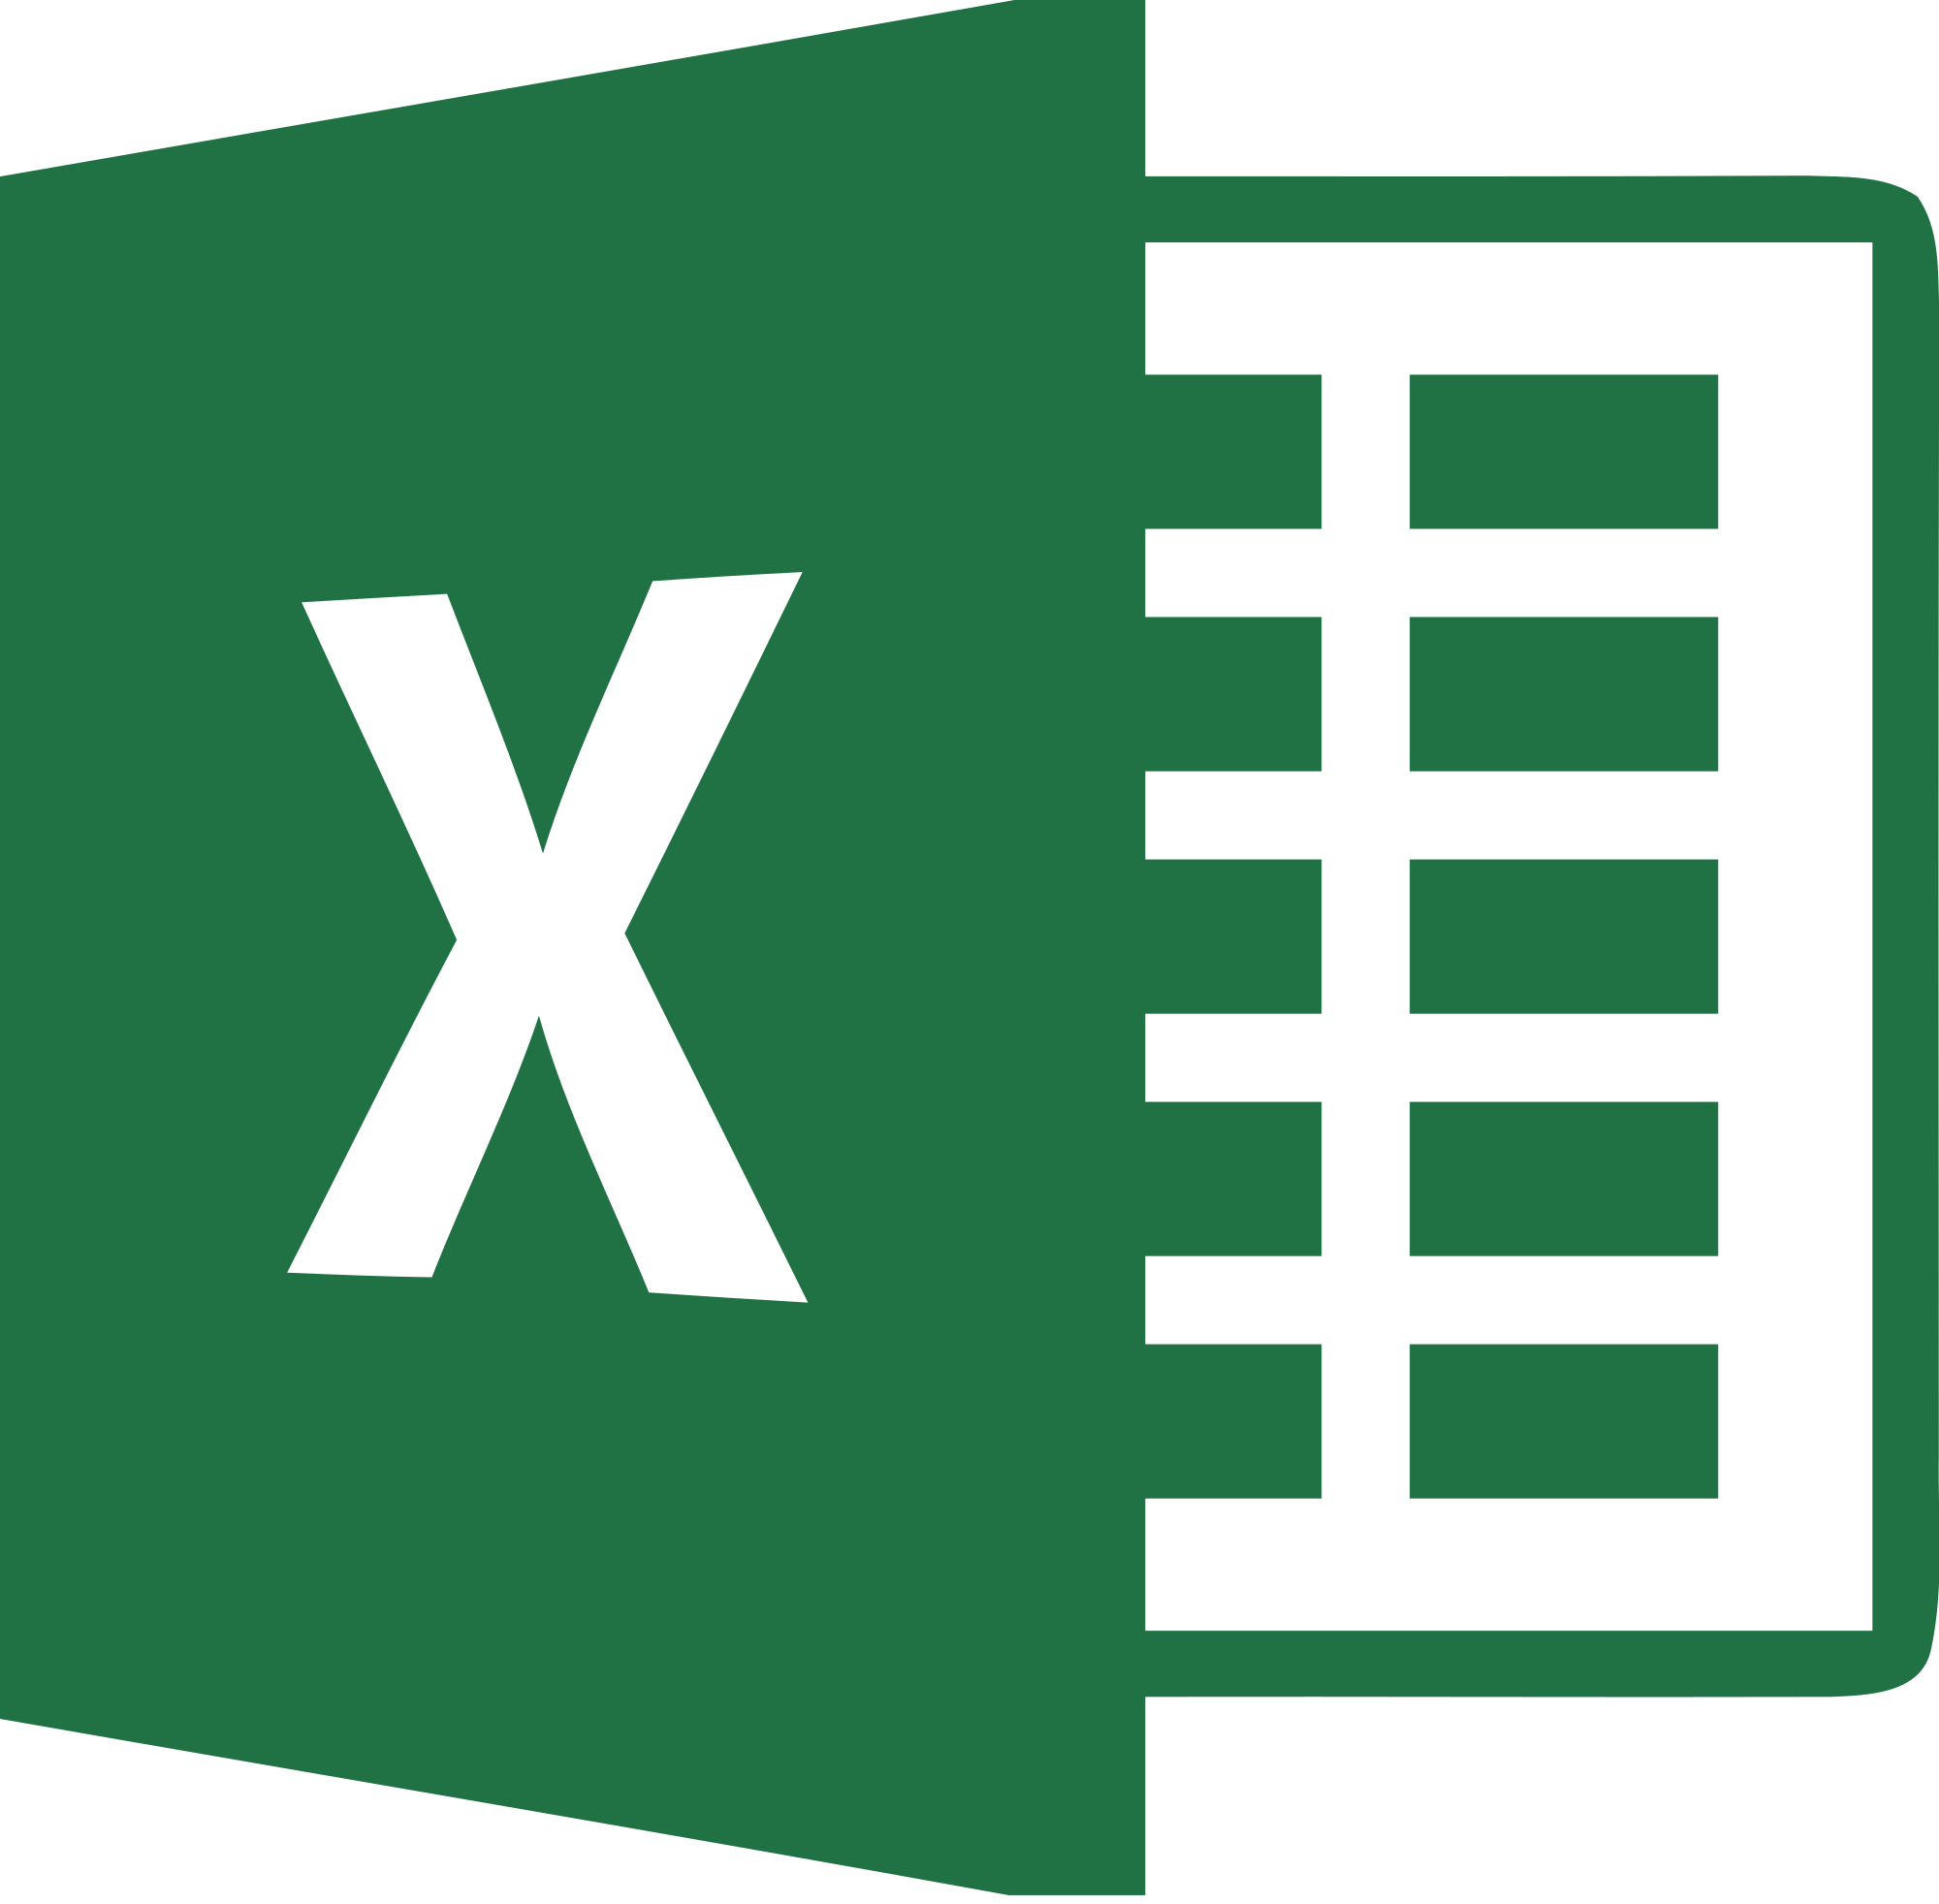
\includegraphics[scale=0.012, trim=0 25cm 0 0]{excel.png} \\\vspace{0.35cm} \emph{R is powerful, but spreadsheets are easier to use.}
	    \end{itemize}
    \end{block}

\end{frame}
